\documentclass{article}[12pt, a4paper]
\topmargin = 15pt

\usepackage{graphics}
\usepackage[top=1.25in, bottom=1.25in, left=44mm, right=44mm]{geometry}
\usepackage[hidelinks]{hyperref}
\usepackage[utf8]{inputenc}
\usepackage{parskip}

%\VignetteIndexEntry{Downscaling tutorial}
%\vignetteDepends{downscale}

\graphicspath{{figures/}}






\usepackage{Sweave}
\begin{document}
\Sconcordance{concordance:Downscaling.tex:Downscaling.Rnw:%
1 22 1 1 6 1 1 1 0 998 1}


\title{Downscaling species occupancy: \\ an introduction and tutorial}
\author{Charles J. Marsh}
\date{\today}
\maketitle

\section{Introduction to downscaling}

In order to assess and manage the status of a species we need to know the abundance of individuals in the population(s) and their changes over time. For the vast majority of species this information is unobtainable, however one important proxy of true abundance and extinction risk is the area occupied by the species. For example, the area of occupancy (AOO) is a little-used measure of conservation status in the IUCN red list (IUCN 2014). Although easier to estimate than true abundance, the difficulty in estimating AOO lies in the extensive sampling required across the full range of the species at a grain size sufficiently fine to give meaningful estimates (and this grain size may vary with taxa, habitat or region). For the majority of species this is still impractical or unfeasible at these grain sizes. However, as we estimate occupancy at increasing grain sizes we increase our confidence in our presence-absence predictions. Such coarse-grain atlas data, generally generated from opportunistic recording over extended periods of time are much more widely available, however, at such coarse grain sizes we also lose resolution in our status estimates as occupancy rates at large grain sizes are less closely correlated with true abundance (Hartley and Kunin 2003).

A solution is to employ the occupancy-area relationship (OAR), that is the increase in the  area occupied by a species increases as grain size increases (Kunin 1998). If the relationship can be described for occupancy at these coarser grain sizes, where confidence is high, then we can extrapolate the occupancy predictions to the fine grain sizes necessary for conservation assessments that are more closely related to the true abundance, distribution and conservation status.

Many models have been proposed to model this geometric relationship, and it appears that no one model consistently provides the best predictions (Azaele et al. 2012, Barwell et al. 2014). This package provides functions for ten commonly applied models, along with functions for preparing coarse-scale data, plotting results, and an ensemble method for running multiple models and averaging their predictions.

\section{Using the downscale package}

The general flow of the \texttt{downscale} package is presented in fig. \ref{fig:Flow}. Ten downscaling models are available (Nachman, power law, logistic, poisson, negative binomial, generalised negative binomial, improved negative binomial, finite negative binomial, Thomas and Hui models). Details of all models can be found in the help files, and in the supplementary information of Barwell et al. 2014. 

\begin{figure}[!t]
\centering
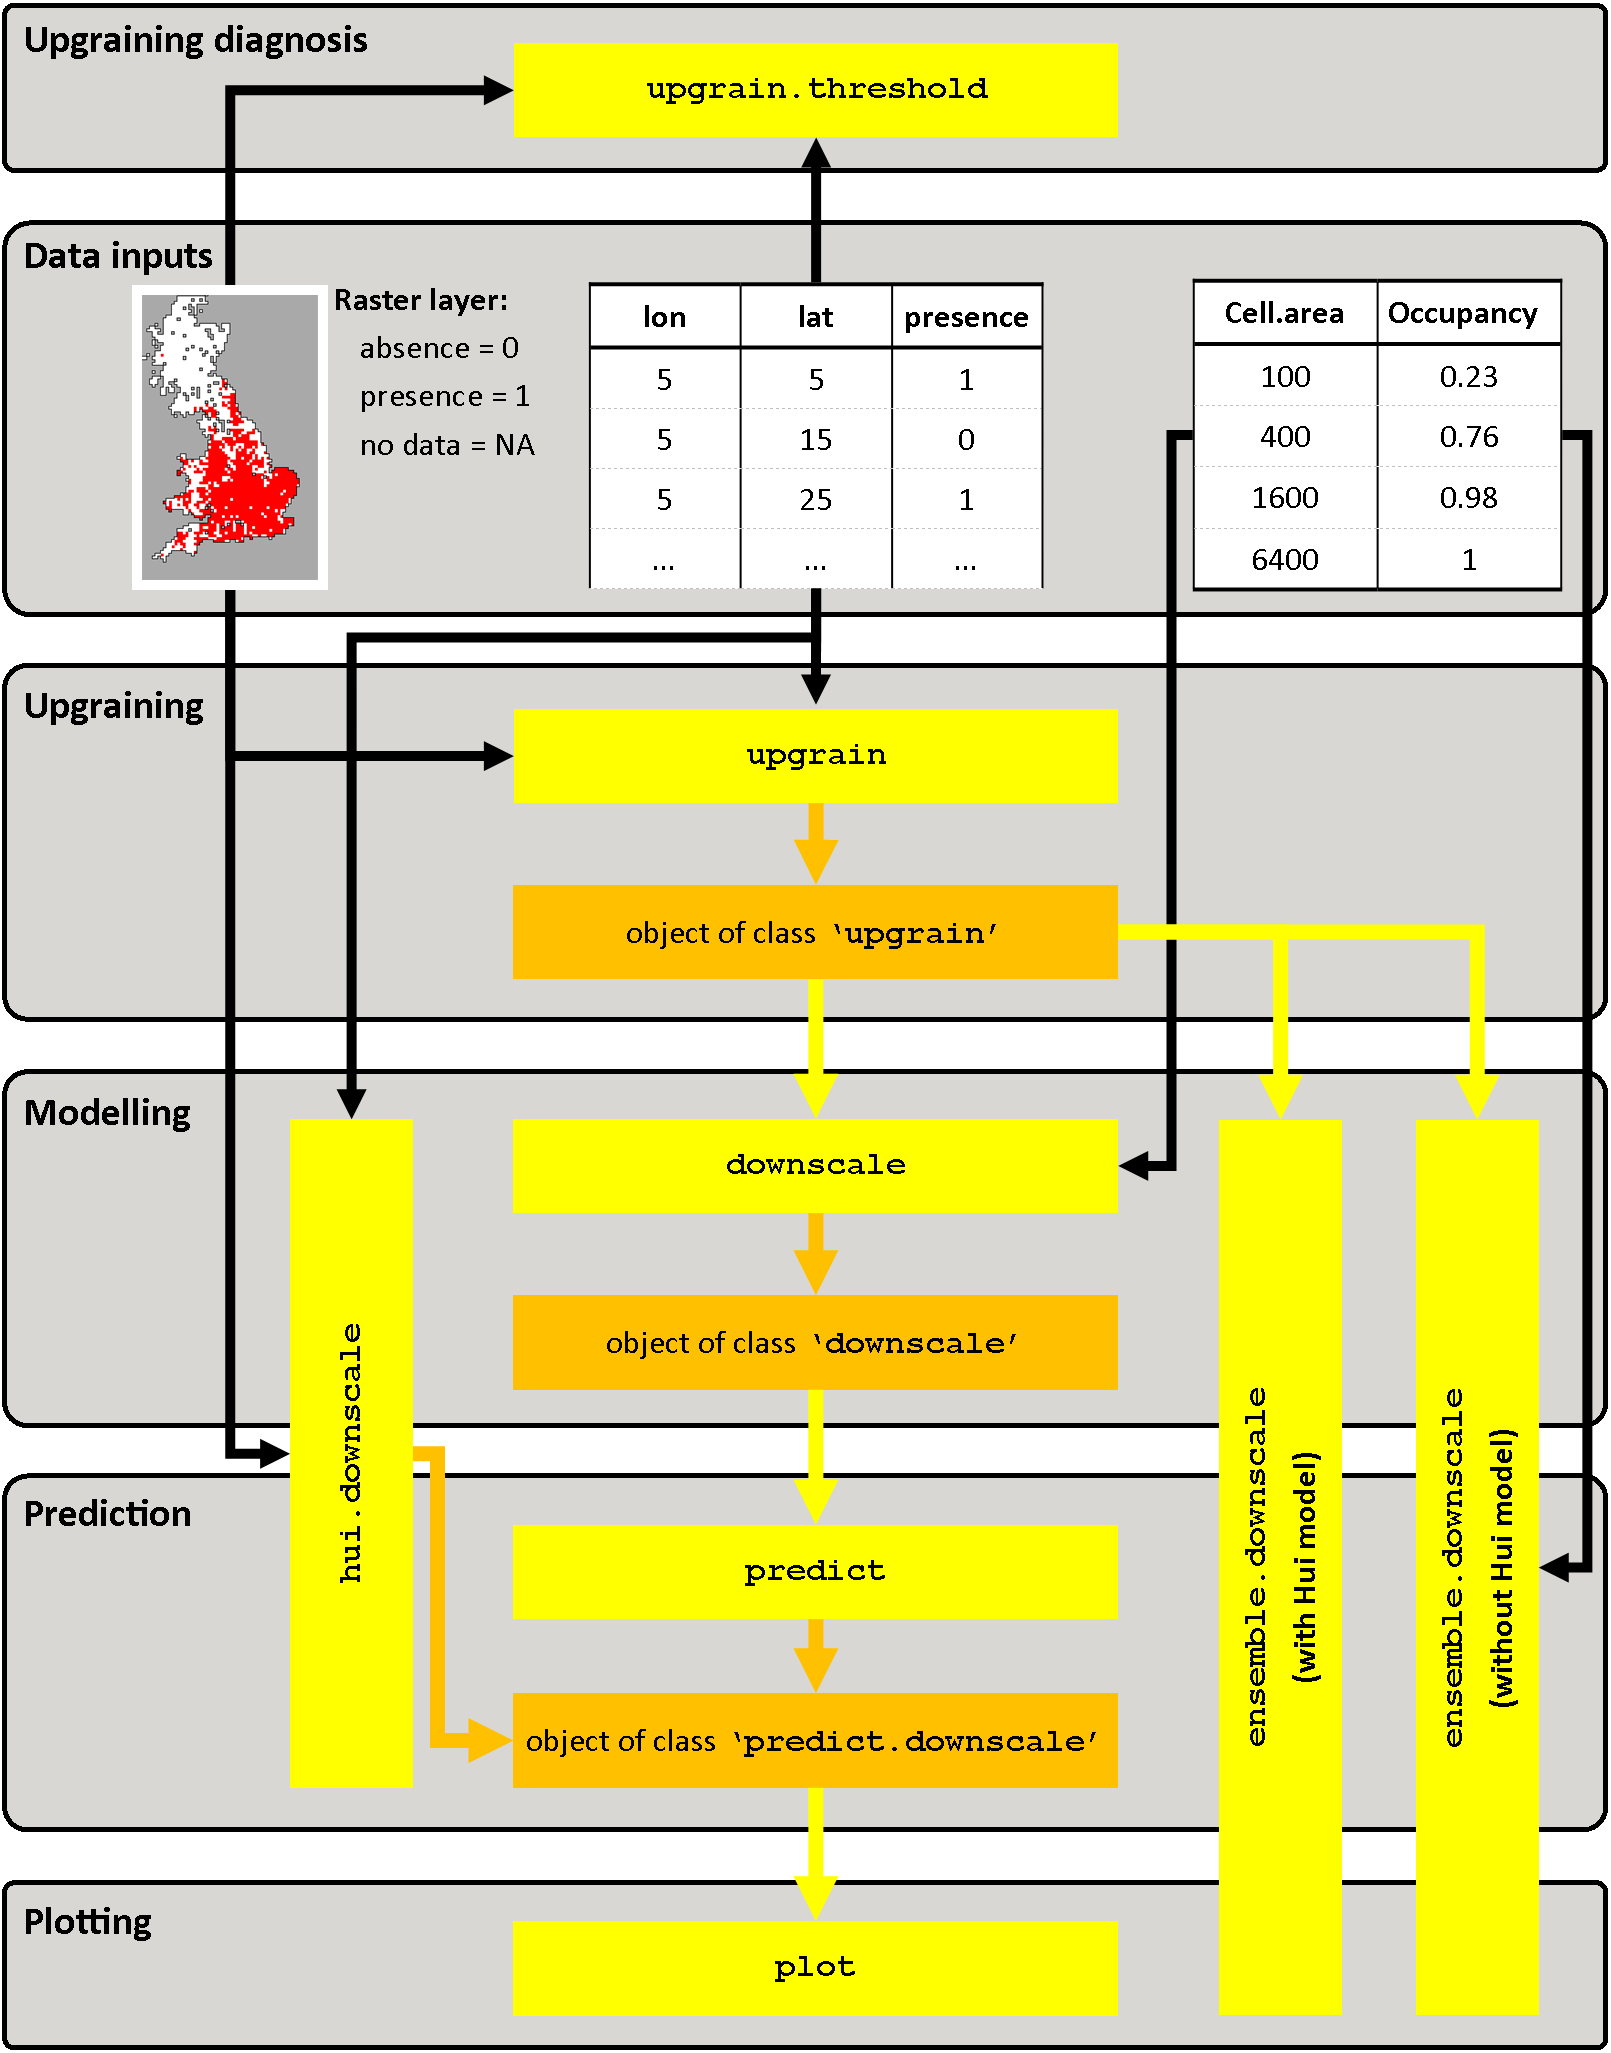
\includegraphics[width=\linewidth]{Flow.png}
\caption{Structure of the \texttt{downscale} package showing all eight functions (yellow) and the three output object classes (orange).}
\label{fig:Flow}
\end{figure}

The user may input three types of data:
\begin{enumerate} \itemsep1pt \parskip0pt 
\item [1)] A data frame of grain sizes (cell area) and occupancies in that order;
\item [2)] A data frame of sample (cell) coordinates and presence-absence data (presence = 1; absence = 0). Column names must be “lon”, “lat”, and “presence”;
\item [3)] 3)  A raster layer of presence-absence data (presence = 1; absence = 0; no data = NA).
\end{enumerate}

If the user wishes to carry out downscaling with the Hui model (Hui et al. 2006, 2009) or upgraining of atlas data (and exploration of upgraining thresholds) then the input data must be of type 2 or 3. Table 1 shows the functions to use to achieve desired objectives with regards to input data.

\begin{table}[!h]
\begin{tabular}{| p{3.9cm} | p{3.5cm} | p{4.1cm} |}
\hline
\textbf{Input data type} & \textbf{Objective} & \textbf{Function flow}  \\\hline
Data frame of cell areas and occcupancies & Downscale (excluding Hui model) & \parbox[t]{0.1cm}{ \texttt{downscale}\Rightarrow \ \texttt{predict}\Rightarrow \ \texttt{plot}}
\\\hline
Data frame of cell coordinates and presence-absence data & Downscale (excluding Hui model) & \parbox[t]{0.1cm}{ \texttt{upgrain.threshold}\Rightarrow\ \texttt{upgrain} \Rightarrow\  \texttt{downscale}\Rightarrow\ \texttt{predict}\Rightarrow\ \texttt{plot}}
\\\hline
Raster layer of presence-absence data & Downscale (excluding Hui model)	& \parbox[t]{0.1cm}{ \texttt{upgrain.threshold}\Rightarrow \ \texttt{upgrain}\Rightarrow \ \texttt{downscale}\Rightarrow \ \texttt{predict}\Rightarrow \texttt{plot}}
\\\hline
Data frame of cell coordinates and presence-absence data &	Downscale (including Hui model)	& \parbox[t]{0.1cm}{ \texttt{hui.downscale}\Rightarrow \ \texttt{plot}}
\\\hline
Raster layer of presence-absence data &	Downscale (including Hui model) &	\parbox[t]{0.1cm}{ \texttt{hui.downscale}\Rightarrow \ \texttt{plot}}
\\\hline
Data frame of cell coordinates and presence-absence data &	Ensemble modelling (excluding Hui model) &	\parbox[t]{0.1cm}{\texttt{ensemble.downscale}}
\\\hline
Raster layer of presence-absence data &	Ensemble modelling (with or without Hui model) &	\texttt{upgrain.threshold}\Rightarrow \ \texttt{upgrain}\Rightarrow \ \texttt{ensemble.downscale}}
\\\hline
\end{tabular}
\caption{Flow of functions for different objectives depending on data input type.}
\end{table}


For downscale modelling it is important they check their data for the scale of saturation and endemism. The scale of saturation is the grain size where all cells are occupied (fig. \ref{fig:Saturation}a). The scale of endemism is the grain size where the entire distribution occurs in a single cell (\ref{fig:Saturation}b). All occupancies above these grain sizes should be set to NA, as they are providing no information for the occupancy-area curve. The downscale functions will automatically set these occupancies to NA for modelling purposes, which can lead to not enough scales remaining for downscaling.

\begin{figure}[!t]
\centering
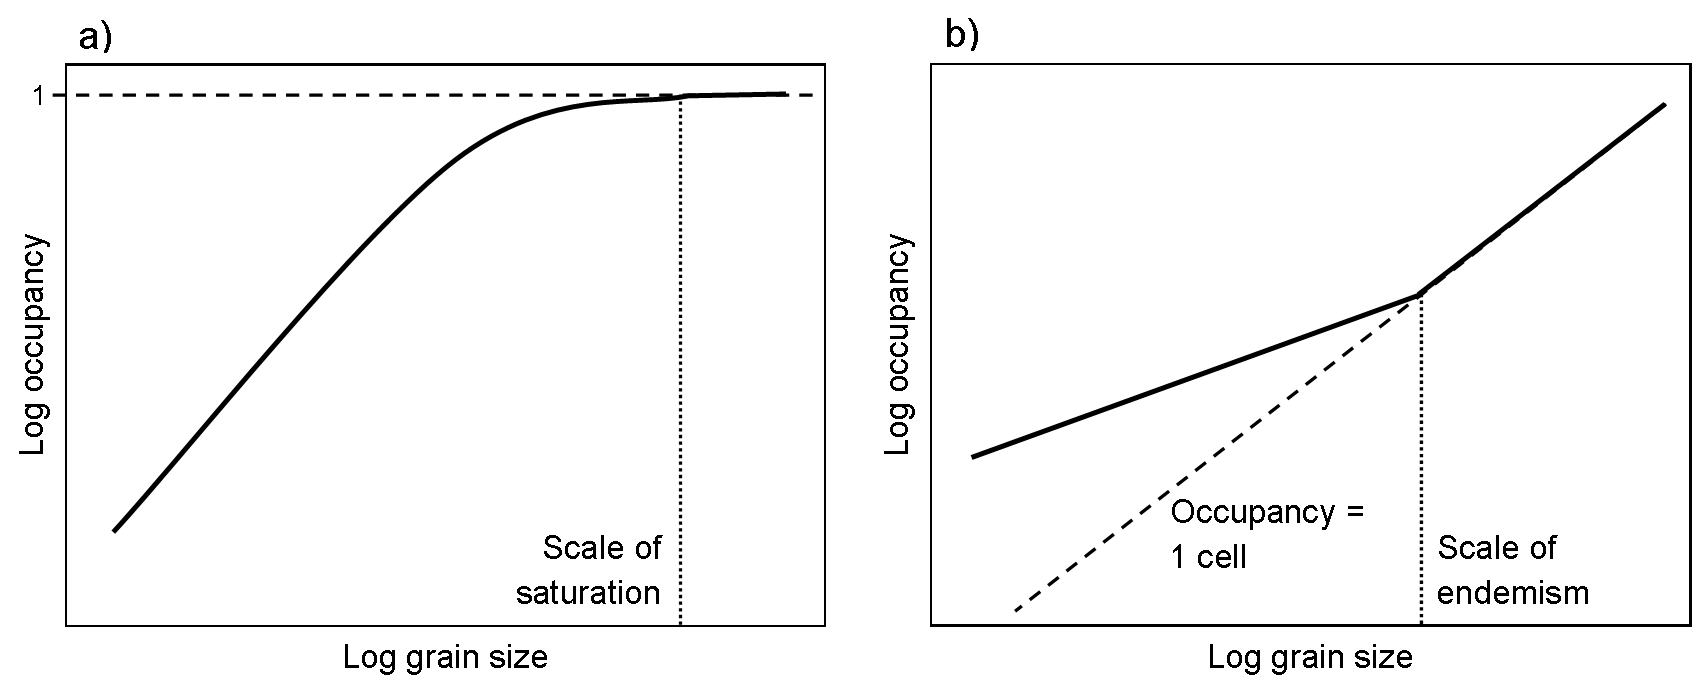
\includegraphics[width=\linewidth]{Saturation.png}
\caption{Occupancy-area relationships for two species showing a) the scale of saturation (the grain size at which all cells are occupied – ie occupancy = 1) and b) the scale of endemism (the scale at which only one cell is occupied). Occupancies of all grain sizes above these points should be set to NA.}
\label{fig:Saturation}
\end{figure}

\section{Package tutorial}

First, we must download the downscale package from R-forge.

\begin{Schunk}
\begin{Sinput}
> install.packages("downscale",
+                  repos = "http://R-Forge.R-project.org")
\end{Sinput}
\end{Schunk}

Then load in the library

\begin{Schunk}
\begin{Sinput}
> library("downscale")
\end{Sinput}
\end{Schunk}

\subsection{A quick example}
We will start with the simplest example of using the downscaling package, where we already have occupancy data across a number of spatial scales (grain size). In this tutorial, we’ll create some dummy data; a data frame where the first column are the cell areas (grain size) and the proportion of occupancy as the second column:

\begin{Schunk}
\begin{Sinput}
> occupancy <- data.frame(Cell.area = c(100, 400, 1600, 6400),
+                         Occupancy = c(0.23, 0.56, 0.87, 1))
\end{Sinput}
\end{Schunk}

Now we use downscale to estimate the model parameters for the logistic model to the data (note: for this type of data input we must also specify the total extent):

\begin{Schunk}
\begin{Sinput}
> logis.mod <- downscale(occupancies = occupancy,
+                        model = "Logis",
+                        extent = 320000)
> ## this creates an object of class ‘downscale’
> logis.mod
\end{Sinput}
\begin{Soutput}
$model
[1] "Logis"

$pars
          C           z 
0.002014927 1.083725424 

$observed
  Cell.area Occupancy
1       100      0.23
2       400      0.56
3      1600      0.87
4      6400      1.00

$extent
[1] 320000

attr(,"class")
[1] "downscale"

\end{Soutput}
\end{Schunk}

Using the modelled parameters from the \texttt{‘downscale’} object we can predict occupancies at finer grain sizes. We will first create a vector of cell sizes (area) to predict. If we include the original cell sizes used for modelling we can also observe the model fit.

\begin{Schunk}
\begin{Sinput}
> areas.pred <- c(1, 2, 5, 25, 100, 400, 1600, 6400)
> logis.pred <- predict(logis.mod,
+                       new.areas = areas.pred)
> ## this creates an object of class ‘predict.downscale’
> ## occupancy is given as a proportion and area of occupancy (AOO)
> logis.pred$predicted
\end{Sinput}
\begin{Soutput}
  Cell.area   Occupancy         AOO
1         1 0.002010876    643.4802
2         2 0.004252482   1360.7942
3         5 0.011396541   3646.8932
4        25 0.061873397  19799.4871
5       100 0.228564935  73140.7793
6       400 0.570999511 182719.8435
7      1600 0.856717834 274149.7068
8      6400 0.964106833 308514.1867

\end{Soutput}
\end{Schunk}
\begin{Schunk}
\begin{Sinput}
> ## now we can plot the predictions
> plot(logis.pred)
\end{Sinput}
\end{Schunk}
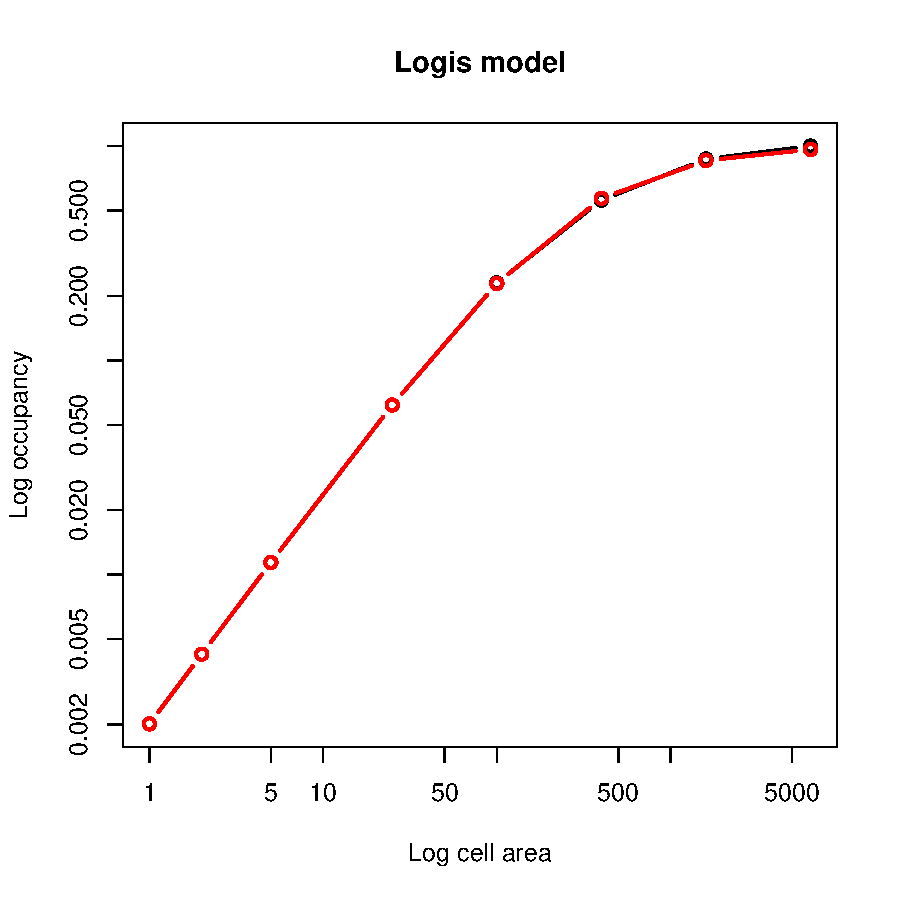
\includegraphics{Downscaling-downscale6}

\subsection{Using atlas data}
For the majority of cases we will only have atlas data that first needs to be upgrained. Read in example atlas data for the UK (in this case a data frame of sample cell coordinates and presence-absence data):

\begin{Schunk}
\begin{Sinput}
> ## if it is not already loaded, load in the package
> library(downscale)
> data.file <- system.file("extdata", "atlas_data.txt", package = "downscale")
> atlas.data <- read.table(data.file, header = TRUE)
\end{Sinput}
\end{Schunk}

The data frame must have the column names “lon”, “lat” and “presence”:

\begin{Schunk}
\begin{Sinput}
> head(atlas.data)
\end{Sinput}
\begin{Soutput}
   lon lat presence
1 8170  10        0
2 8130  20        0
3 8140  20        0
4 8160  20        0
5 8170  20        0
6 8140  30        0

\end{Soutput}
\end{Schunk}

The first step is to upgrain the atlas data to calculate occupancy at larger grain sizes than the atlas data – this provides the proportion of occupancy data points to fit the different downscaling models to. Therefore it is important that we fix the extent for all grain sizes, but this means compromising between assigning unsampled cells as absences or excluding sampled cells as No Data. We can explore this trade-off with \texttt{upgrain.threshold}:

\begin{Schunk}
\begin{Sinput}
> ## explore thresholds using upgrain.threshold
> thresh <- upgrain.threshold(atlas.data = atlas.data,
+                             cell.width = 10,
+                             scales = 3,
+                             thresholds = seq(0, 1, 0.01))
> ## see the four optional thresholds
> thresh$Thresholds
\end{Sinput}
\begin{Soutput}
  All_Sampled All_Occurrences Gain_Equals_Loss Sampled_Only
1           0            0.04             0.51            1

\end{Soutput}
\end{Schunk}

\begin{figure}[!h]
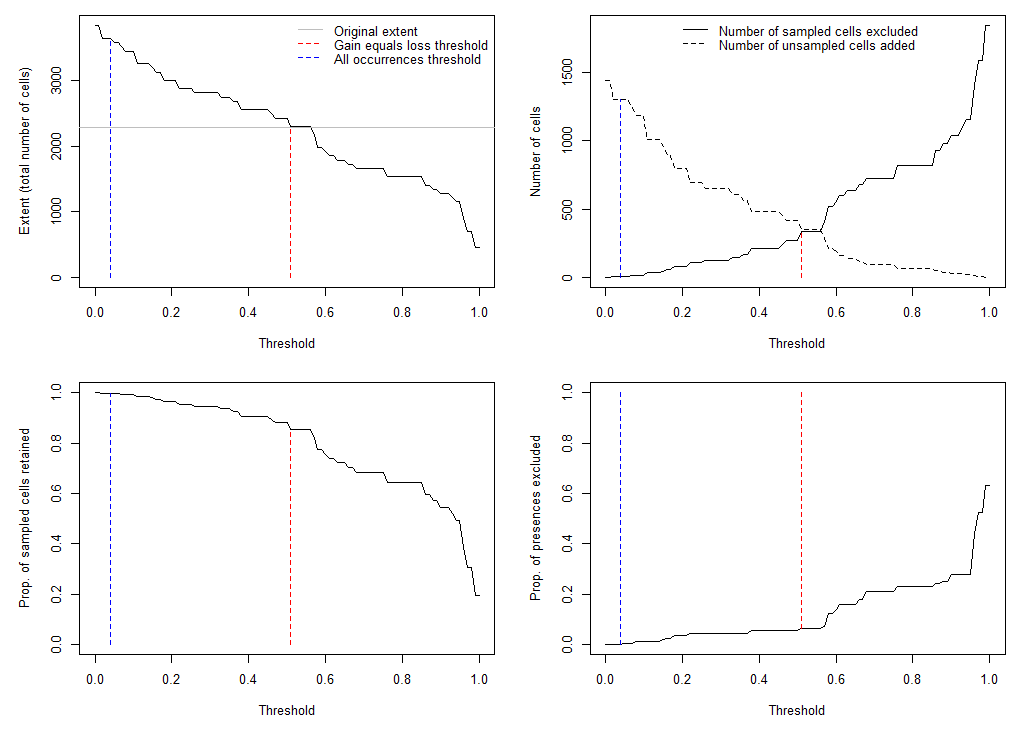
\includegraphics[width=\linewidth]{Threshold_plots.png}
\end{figure}

\begin{figure}[!]
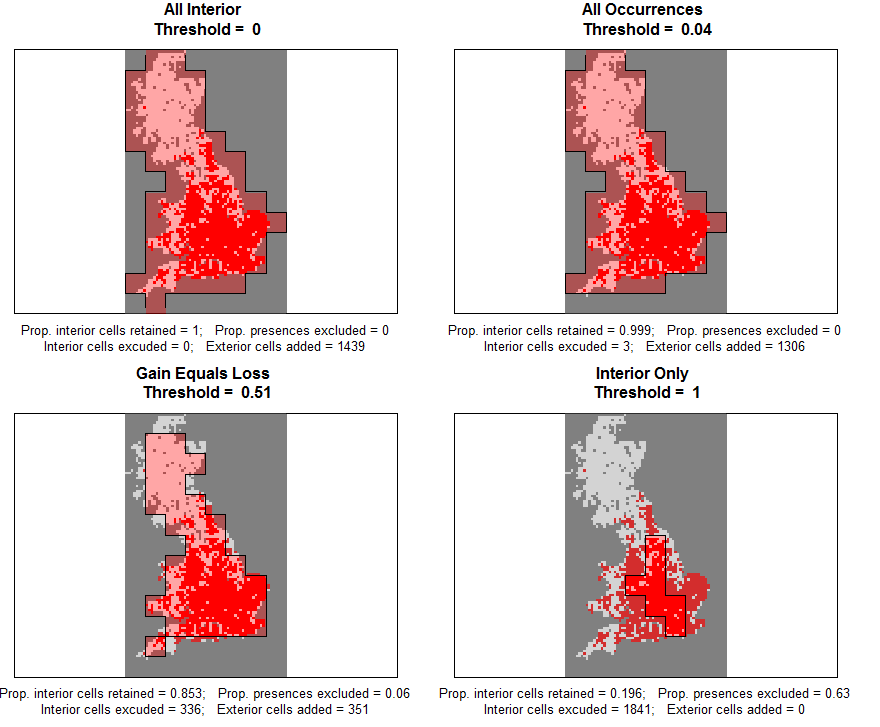
\includegraphics[width=\linewidth]{Threshold_maps.png}
\end{figure}

This gives two sets of plots (hit \texttt{return} or click on the plot window to see the second set). The first are a set of four plots that explore the trade-offs, and the second set are the standardised atlas data generated after applying four different threshold criteria ("All Sampled",  "All Presences",  "Gain Equals Loss" and "Sampled Only"). It is highly recommended to read the vignette “Upgraining atlas data for downscaling: threshold selection using upgrain.threshold” for more detail on creating your cross-scale standardised atlas data:

\begin{Schunk}
\begin{Sinput}
>   vignette("Upgraining", package = "downscale")
\end{Sinput}
\end{Schunk}

The user can input any threshold they wish, but for now we’ll use one of the pre-defined options “All Presences” which ensures that all presence records are maintained:

\begin{Schunk}
\begin{Sinput}
> ## upgrain data (using All Presences threshold)
> occupancy <- upgrain(atlas.data,
+                      cell.width = 10,
+                      scales = 3,
+                      method = "All_Presences")
\end{Sinput}
\end{Schunk}
\includegraphics{Downscaling-downscale11}

This creates an object of class \texttt{‘upgrain’} which can then be used directly as an input for downscaling.

\subsection{Downscaling - more detailed examples}

Fitting the downscaling models is as before, except that we no longer require to input the extent, which is passed directly from \texttt{‘upgrain’}. Let’s try the improved negative binomial model (INB):

\begin{Schunk}
\begin{Sinput}
> ## if it is not already loaded, load in the package
> library(downscale)
> ## Improved Negative Binomial model
> (inb <- downscale(occupancies = occupancy,
+                   model = "INB"))
\end{Sinput}
\begin{Soutput}
$model
[1] "INB"

$pars
         C          r          b 
1.42670491 0.04906771 1.82970792 

$observed
  Cell.area Occupancy
1       100 0.2713542
2       400 0.4122807
3      1600 0.5219298
4      6400 0.7017544

$extent
[1] 364800

attr(,"class")
[1] "downscale"

\end{Soutput}
\end{Schunk}

The downscaling functions use an optimisation procedure to fit the models to the upgrained occupancy data. Suitable starting values for model parameters are automatically inputted, however if the models aren’t converging then it is possible to specify user-specific parameters. They must be in the form of a list with the same parameter names (take particular note of capitals) as the original starting parameters:

\begin{Schunk}
\begin{Sinput}
> ## Specifying the starting parameters
> params.new <- list("C" = 0.1, "r" = 0.00001, "b" = 0.1)
> (inb.new <- downscale(occupancies = occupancy,
+                       model = "INB",
+                       starting_params = params.new))
\end{Sinput}
\begin{Soutput}
$model
[1] "INB"

$pars
            C             r             b 
 1.161747e-28  1.669658e-05 -3.712604e-01 

$observed
  Cell.area Occupancy
1       100 0.2713542
2       400 0.4122807
3      1600 0.5219298
4      6400 0.7017544

$extent
[1] 364800

attr(,"class")
[1] "downscale"

\end{Soutput}
\end{Schunk}

Table 2 shows the default starting parameters implemented.

\begin{table}[!h]
\centering
\begin{tabular}{| l | l | l | l |}
\hline
\textbf{Model} & \textbf{Parameter 1} &	\textbf{Parameter 2} &	\textbf{Parameter 3} \\\hline
Nachman &	"C" = 0.01 &	"z" = 0.01 & \\	
PL &	"C" = 0.01 &	"z" = 0.01 & \\
Logis &	"C" = 0.01 &	"z" = 0.01 & \\	
Poisson &	"lambda" = 1e-8 &  &	\\
NB &	"C" = 0.01 &	"k" = 0.01 & \\	
GNB	& "C" = 0.00001 &	"z" = 1 &	"k" = 0.01 \\
INB	& "C" = 1 &	"r" = 0.01 &	"b" = 0.1 \\
FNB	& "W" = 10 &	"k" = 10 & \\	
Thomas &	"rho" = 1e-8 &	"mu" = 10 &	"sigma" = 1 \\\hline
\end{tabular}
\label{table:pars}
\end{table}

We can visually compare the two to see which has a better fit (plotting can be called directly from \texttt{predict} or through \tetxttt{plot}):

\begin{Schunk}
\begin{Sinput}
> ## plot the predictions of two FNB models using predict.downscale
> ind.pred <- predict(inb,
+                     new.areas = c(1, 2, 5, 25, 100, 400, 1600, 6400),
+                     plot = TRUE)
> inb.pred.new <- predict(inb.new,
+                         new.areas = c(1, 2, 5, 25, 100, 400, 1600, 6400),
+                         plot = TRUE)
\end{Sinput}
\end{Schunk}
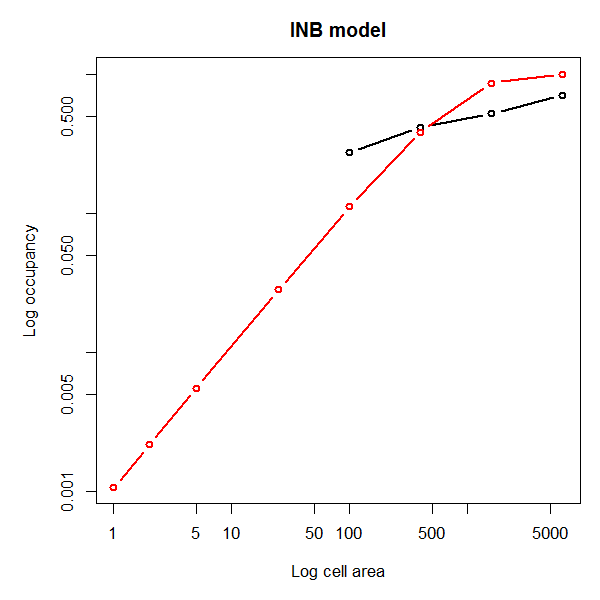
\includegraphics{Downscaling-downscale14}

The Thomas model involves an integration process that can be time-consuming to run. For this reason the user may select tolerance during integration – the finer the tolerance, the more accurate the prediction. It can therefore be a good idea to initially try a larger tolerance value in order to ascertain if the starting parameters are likely to be correct.

\begin{Schunk}
\begin{Sinput}
> ## Thomas model
> thomas <- downscale(occupancies = occupancy,
+                     model = "Thomas",
+                     tolerance = 1e-3)
> ## the tolerance can also be set for the predict function
> thomas.pred <- predict(thomas,
+                        new.areas = c(1, 2, 5, 25, 100, 400, 1600, 6400),
+                        tolerance = 1e-6)
\end{Sinput}
\end{Schunk}
\begin{Schunk}
\begin{Sinput}
> ## When plotting the results we can change the graphics
> plot(thomas.pred,
+      col.pred = "green",
+      pch = 16,
+      lwd.obs = 3)
\end{Sinput}
\end{Schunk}
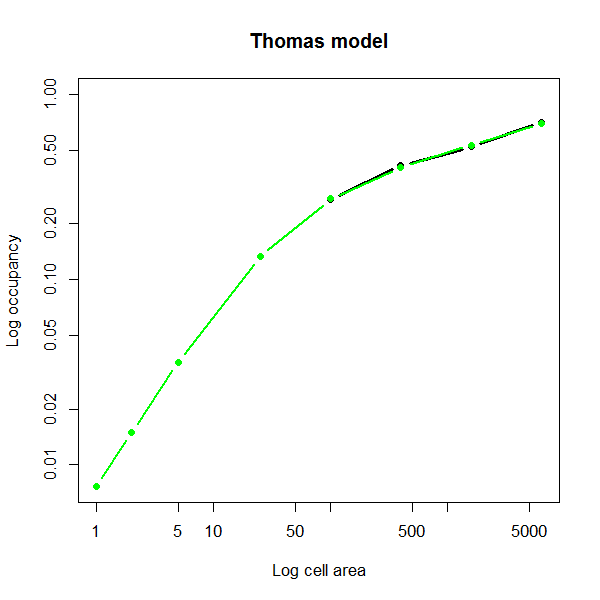
\includegraphics{Downscaling-downscale16}

The Hui model is slightly different from the other downscaling models in that it does not need occupancy from multiple scales. Instead, it only takes the data from the atlas scale and uses this to calculate occupancy at finer grain sizes – in effect the hui.downscale function runs downscale and predict.downscale in one step. Therefore the input data must either be a presence-absence raster layer of the atlas data, or a data frame of cell coordinates and presence-absence data. Additionally the function requires the cell widths of the input data, along with the grain size (cell area) for which we wish to predict occupancy. These must be smaller than the cell area of the input data. Additionally, like the Thomas model, the tolerance can be specified if the results appear inaccurate (set tolerance to a smaller number) or takes extensive programming time (set tolerance to a larger number).

\begin{Schunk}
\begin{Sinput}
> ## Hui model
> hui <- hui.downscale(atlas.data,
+                      cell.width = 10,
+                      new.areas = c(1, 2, 5, 15, 50))
\end{Sinput}
\end{Schunk}
\begin{Schunk}
\begin{Sinput}
> ## the output is a normal ‘predict.downscale’ object	
> plot(hui)
\end{Sinput}
\end{Schunk}
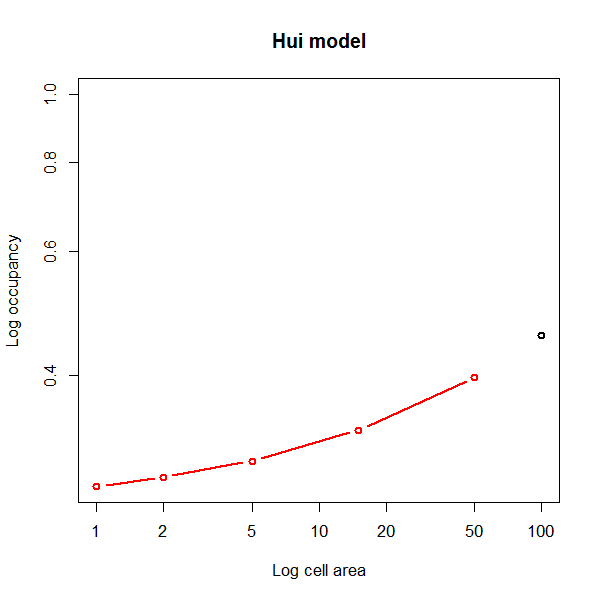
\includegraphics{Downscaling-downscale18}

\subsection{Ensemble modelling}
It is probable that the user won’t know which model will provide the most accurate predictions. Therefore there is an ensemble function that will model and predict occupancy for multiple models simultaneously. It also applies a simple model averaged prediction (the means of the log occupancies). Some or all of the models can be selected. If we don’t wish to run the Hui model input data can be a data frame of occupancies and cell areas, along with the grain sizes we wish to predict and the total extent:

\begin{Schunk}
\begin{Sinput}
> ## if it is not already loaded load in the package
> library(downscale)
> ## hypothetical occupancy data
> occupancy <- data.frame(Cell.area = c(100, 400, 1600, 6400),
+                         Occupancy = c(0.23, 0.56, 0.87, 1))
> ## grain sizes (cell areas) to predict
> areas.pred <- c(1, 2, 5, 25, 100, 400, 1600, 6400)
\end{Sinput}
\end{Schunk}
\begin{Schunk}
\begin{Sinput}
> ensemble <- ensemble.downscale(occupancy,
+                                new.areas = areas.pred,
+                                extent = 320000,
+                                models = c("Nachman",
+                                           "PL",
+                                           "Logis",
+                                           "GNB",
+                                           "FNB"),
+                                plot = TRUE)
\end{Sinput}
\begin{Soutput}
Nachman model is running...  complete 
PL model is running...  complete 
Logis model is running...  complete 
GNB model is running...  complete 
FNB model is running...  complete 

\end{Soutput}
\end{Schunk}
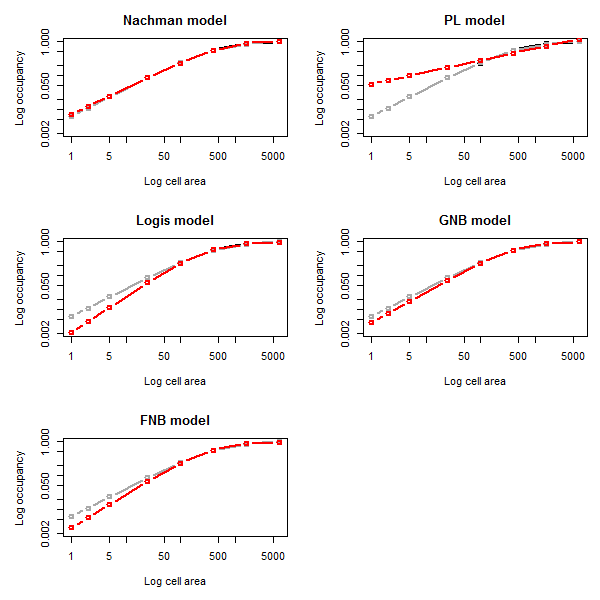
\includegraphics{Downscaling-downscale}
\begin{Schunk}
\begin{Sinput}
> ## the model averaged predictions are in grey
> ## predicted proportion of occupancies
> ensemble$Occupancy
\end{Sinput}
\begin{Soutput}
  Cell.area     Nachman         PL       Logis         GNB
1         1 0.007084977 0.05581996 0.002010876 0.004059485
2         2 0.012179638 0.07113722 0.004252482 0.007645696
3         5 0.024851808 0.09801796 0.011396541 0.017587267
4        25 0.085220244 0.17211624 0.061873397 0.073735530
5       100 0.232474679 0.27953528 0.228564935 0.230188967
6       400 0.544305709 0.45399534 0.570999511 0.558122075
7      1600 0.903148404 0.73733723 0.856717834 0.877387332
8      6400 0.999026625 1.19751493 0.964106833 0.984486991
          FNB       Means
1 0.002840894 0.006201373
2 0.005668054 0.010981077
3 0.014068055 0.023300961
4 0.067107408 0.085204625
5 0.228575983 0.239104306
6 0.566654658 0.536927362
7 0.870161429 0.846858509
8 0.976325167 1.020839639

\end{Soutput}
\begin{Sinput}
> ## predicted area of occupancies (AOO)
> ensemble$AOO
\end{Sinput}
\begin{Soutput}
  Cell.area    Nachman        PL       Logis        GNB
1         1   2267.193  17862.39    643.4802   1299.035
2         2   3897.484  22763.91   1360.7942   2446.623
3         5   7952.579  31365.75   3646.8932   5627.925
4        25  27270.478  55077.20  19799.4871  23595.370
5       100  74391.897  89451.29  73140.7793  73660.469
6       400 174177.827 145278.51 182719.8435 178599.064
7      1600 289007.489 235947.91 274149.7068 280763.946
8      6400 319688.520 383204.78 308514.1867 315035.837
          FNB      Means
1    909.0862   1984.439
2   1813.7772   3513.945
3   4501.7776   7456.307
4  21474.3707  27265.480
5  73144.3146  76513.378
6 181329.4907 171816.756
7 278451.6571 270994.723
8 312424.0534 326668.684

\end{Soutput}
\end{Schunk}

Alternatively, the input data may be an object of class \texttt{‘upgrain’}, which also allows us to run the Hui model as long as we specify the cell width:

\begin{Schunk}
\begin{Sinput}
> ## read in atlas data
> data.file <- system.file("extdata", "atlas_data.txt", package = "downscale")
> atlas.data <- read.table(data.file, header = TRUE)
\end{Sinput}
\end{Schunk}
\setkeys{Gin}{width=1\linewidth}
\begin{Schunk}
\begin{Sinput}
> ## upgrain data (using All Presences threshold)
> occupancy <- upgrain(atlas.data,
+                      cell.width = 10,
+                      scales = 3,
+                      method = "All_Presences")
\end{Sinput}
\end{Schunk}
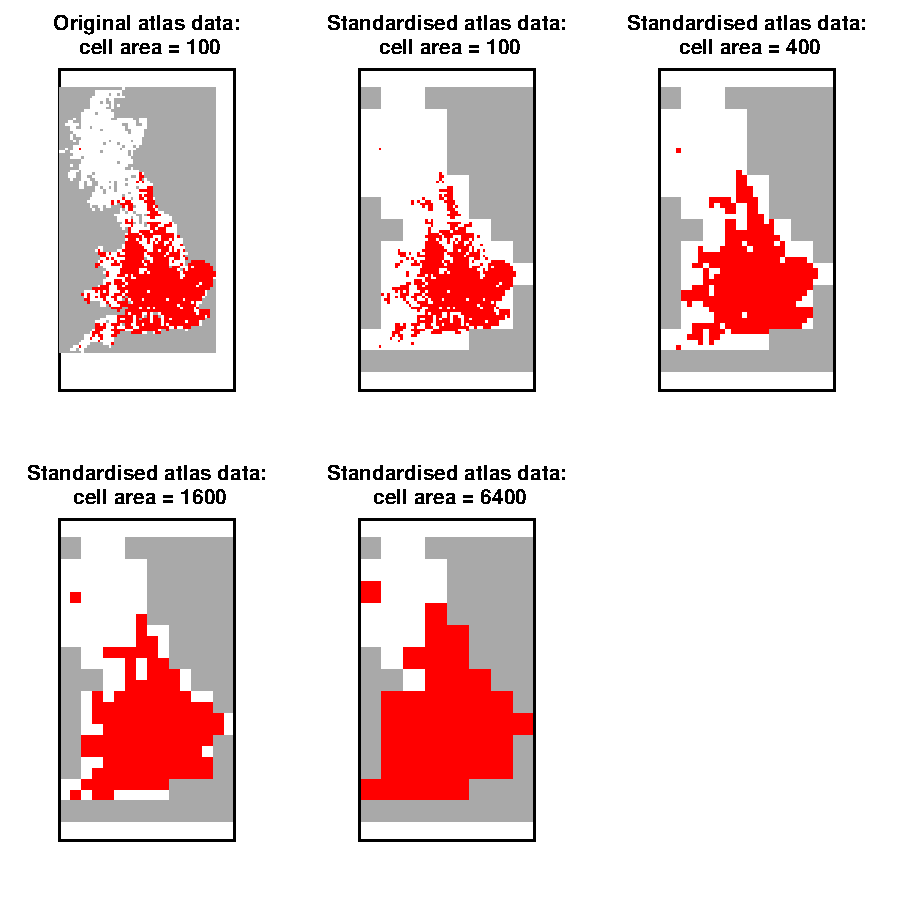
\includegraphics{Downscaling-downscale22}

\setkeys{Gin}{width=0.8\linewidth}
\begin{Schunk}
\begin{Sinput}
> ## ensemble modelling
> ensemble <- ensemble.downscale(occupancy,
+                                new.areas = areas.pred,
+                                cell.width = 10,
+                                models = c("Nachman",
+                                           "PL",
+                                           "Logis",
+                                           "GNB",
+                                           "FNB",
+                                           "Hui"),
+                                plot = TRUE)
\end{Sinput}
\begin{Soutput}
Nachman model is running...  complete 
PL model is running...  complete 
Logis model is running...  complete 
GNB model is running...  complete 
FNB model is running...  complete 
Hui model is running...  complete 

\end{Soutput}
\end{Schunk}
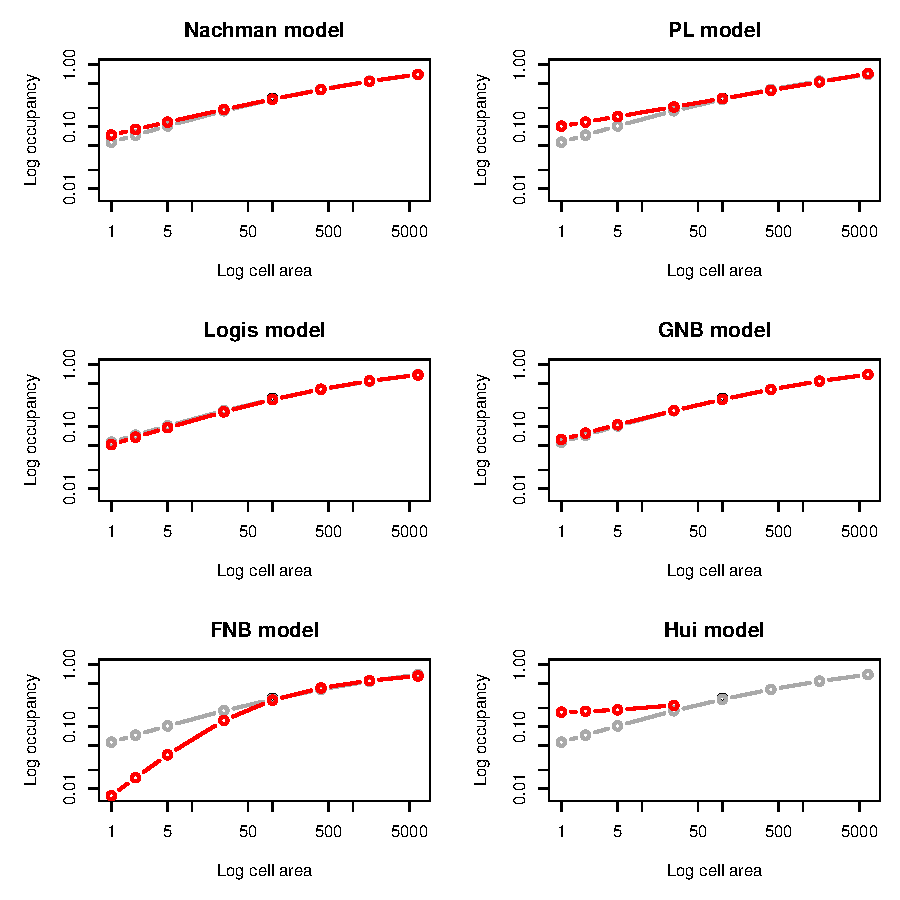
\includegraphics{Downscaling-downscale23}

If we want to run all ten models we can specify \texttt{models = "all"}. Once again, we can set the tolerance values for the modelling (\texttt{tolerance\_mod}) and prediction (\texttt{tolerance\_pred}) of the Thomas model and the Hui model (\texttt{tolerance\_hui}) to improve processing times or accuracy.

\setkeys{Gin}{width=1\linewidth}
\begin{Schunk}
\begin{Sinput}
> ensemble <- ensemble.downscale(occupancy,
+                                new.areas = areas.pred,
+                                cell.width = 10,
+                                models = "all",
+                                tolerance_mod = 1e-3,
+                                plot = TRUE)
\end{Sinput}
\begin{Soutput}
Nachman model is running...  complete 
PL model is running...  complete 
Logis model is running...  complete 
Poisson model is running...  complete 
NB model is running...  complete 
GNB model is running...  complete 
INB model is running...  complete 
FNB model is running...  complete 
Thomas model is running...  complete 
Hui model is running...  complete 

\end{Soutput}
\end{Schunk}
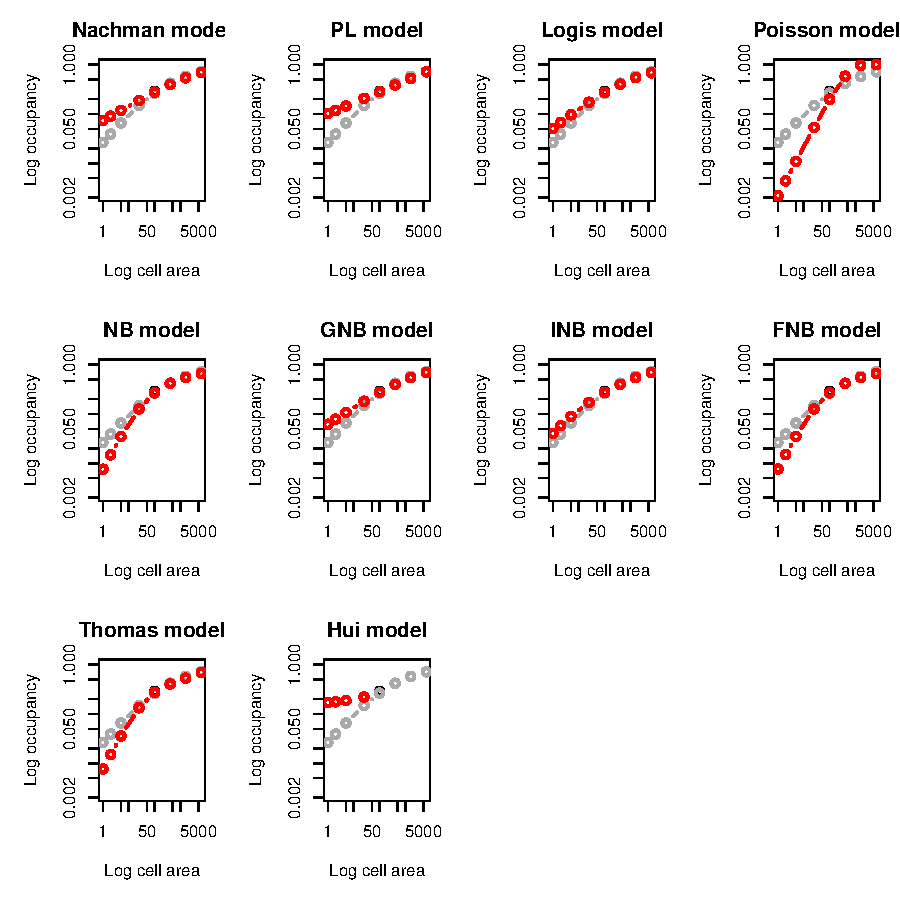
\includegraphics{Downscaling-downscale24}

We can also specify the starting parameters for specific models. For each model the starting parameters should be in the form of a list as before, and each model list is an item in a combined list:

\begin{Schunk}
\begin{Sinput}
> ## Specifying starting parameters for Nachman and GNB models
> new.params <- list(Nachman = list("C" = 0.1, "z" = 0.01),
+                    GNB = list("C" = 0.1, "z" = 1, "k" = 0.01))
> new.params
\end{Sinput}
\begin{Soutput}
$Nachman
$Nachman$C
[1] 0.1

$Nachman$z
[1] 0.01


$GNB
$GNB$C
[1] 0.1

$GNB$z
[1] 1

$GNB$k
[1] 0.01



\end{Soutput}
\end{Schunk}

\begin{Schunk}
\begin{Sinput}
> ensemble <- ensemble.downscale(occupancies = occupancy,
+                                new.areas = c(1, 2, 5, 15, 50, 100, 400, 1600,
+                                              6400),
+                                cell.width = 10,
+                                models = "all",
+                                tolerance_mod = 1e-3,
+                                starting_params = new.params,
+                                plot = TRUE)
\end{Sinput}
\begin{Soutput}
Nachman model is running...  complete 
PL model is running...  complete 
Logis model is running...  complete 
Poisson model is running...  complete 
NB model is running...  complete 
GNB model is running...  complete 
INB model is running...  complete 
FNB model is running...  complete 
Thomas model is running...  complete 
Hui model is running...  complete 

\end{Soutput}
\end{Schunk}
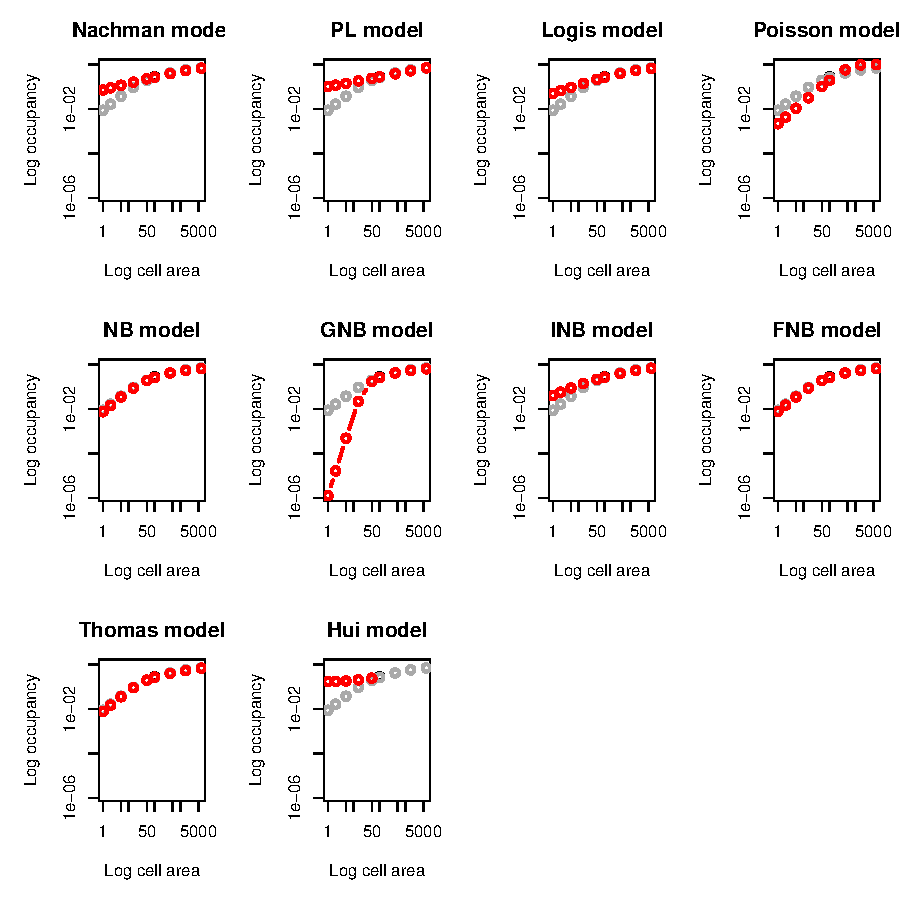
\includegraphics{Downscaling-downscale26}

\subsection{Creating atlas data from point records}

It may be that instead of having pre-existing atlas data, we may need to create our own coarse-scale data from point records (for example herbarium records or GBIF data).

The grain size (cell width) needs to be carefully chosen so that we can best meet the assumption that all cells have been sampled. If there are cells or regions where we do not expect this to be the case it is best to change these to NA’s rather than assign them as absences.

The library \texttt{spocc} will automatically harvest GBIF data for a desired species for a specified region.

\begin{Schunk}
\begin{Sinput}
> library(spocc)
> library(downscale)
\end{Sinput}
\end{Schunk}

We’ll get the records for the chalkhill blue (Polyommatus coridon), a species with a patchy breeding distribution in the UK.

\begin{Schunk}
\begin{Sinput}
> records <- occ(query = "Polyommatus coridon",
+                from = "gbif",
+                limit=10000,
+                gbifopts = list(country ="GB"))
> records <- occ_to_sp(records,
+                      "+proj=longlat +datum=WGS84",
+                      just_coords = TRUE)
> records <- spTransform(records,
+                        CRS("+proj=lcc +lat_1=49.8333339 +lat_2=51.16666733333333
+                            +lat_0=90 +lon_0=4.367486666666666 +x_0=150000.01256 
+                            +y_0=5400088.4378 +ellps=intl +units=km +no_defs"))
\end{Sinput}
\end{Schunk}

We can have a quick look at the point records if we like.

\begin{Schunk}
\begin{Sinput}
> records.coords <- records@coords
\end{Sinput}
\end{Schunk}
\setkeys{Gin}{width=0.8\linewidth}
\begin{Schunk}
\begin{Sinput}
> plot(records.coords)
\end{Sinput}
\end{Schunk}
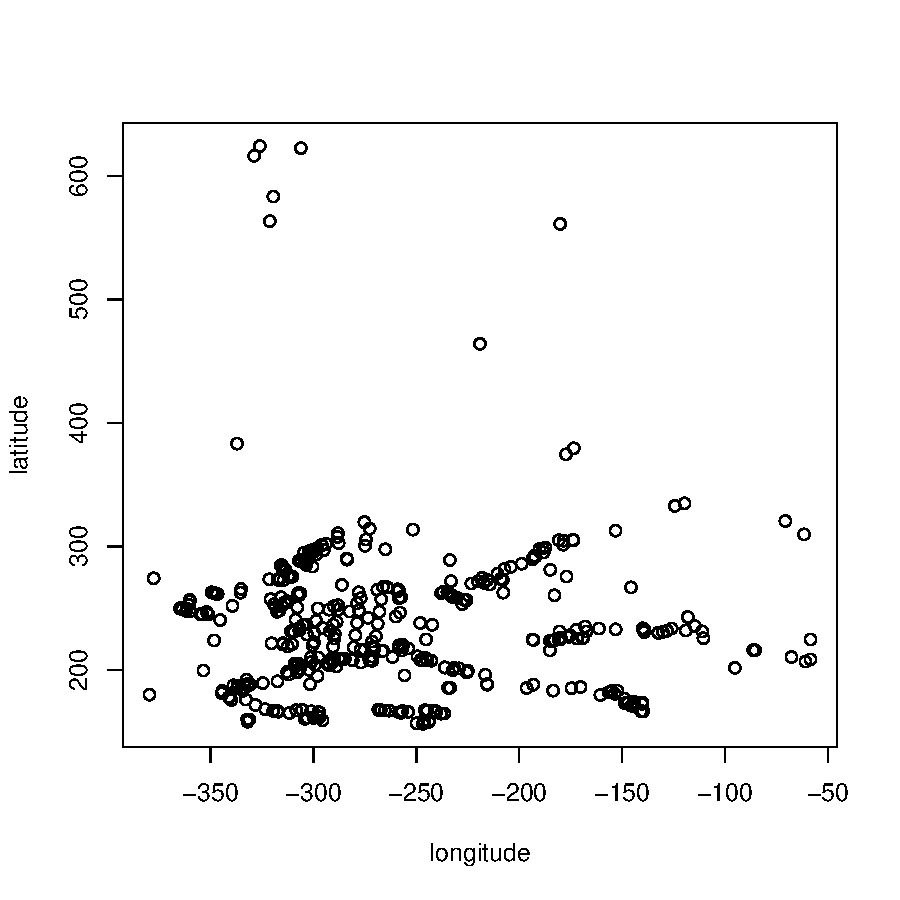
\includegraphics{Downscaling-downscale30}

Now we have to convert these points in to a coarse-scale raster. The simplest method is to bound our raster by the limits of the location coordinates. Careful thought must also be put in to the grain size. It must be large enough that we are confident it is an accurate representation of presence-absence, but also small enough to allow upgraining to give at least three spatial scales worth of occupancy data. Here, as the UK is generally well-sampled, we will set a grain size of 20 km width (400 $km^{2}$), which will still comfortably allow us to upgrain to give three scales (400, 1600, 6400 $km^{2}$).

\begin{Schunk}
\begin{Sinput}
> gbif_raster <- raster(xmn = min(records.coords[, "longitude"]),
+                       xmx = max(records.coords[, "longitude"]),
+                       ymn = min(records.coords[, "latitude"]),
+                       ymx = max(records.coords[, "latitude"]),
+                       res = 20)
> gbif_raster <- rasterize(records, gbif_raster, field = 1)
> ## convert cells with NA (no records) to 0
> gbif_raster[is.na(gbif_raster)] <- 0
\end{Sinput}
\end{Schunk}
\begin{Schunk}
\begin{Sinput}
> plot(gbif_raster)
\end{Sinput}
\end{Schunk}
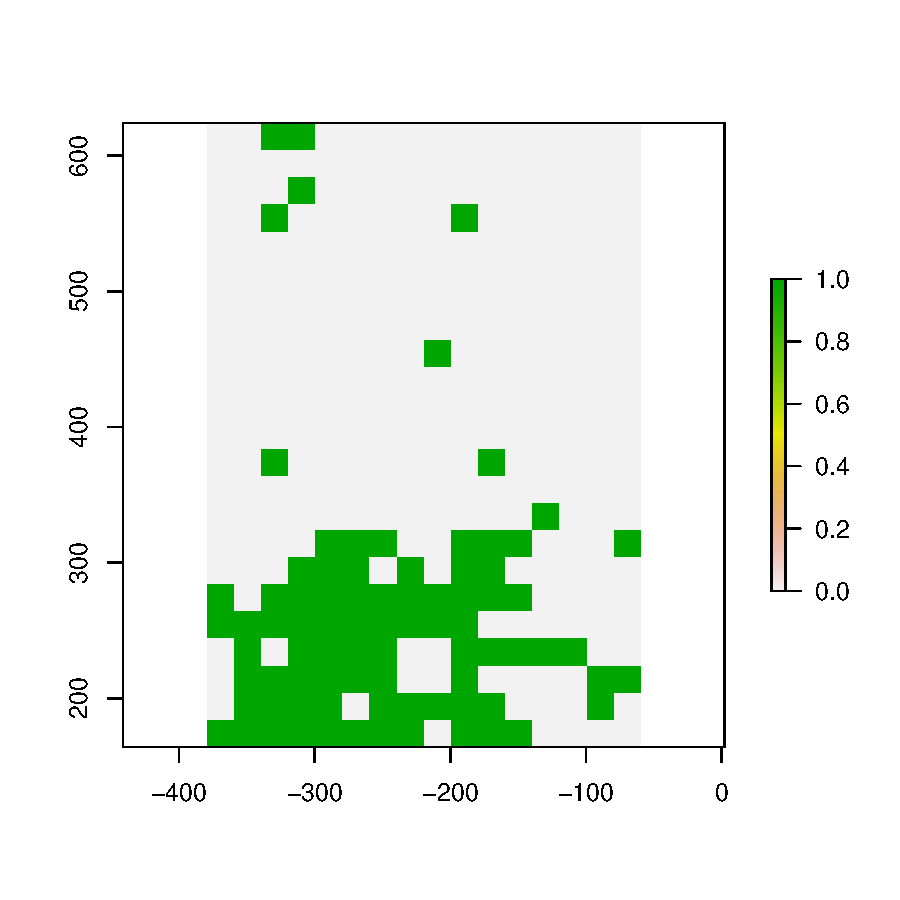
\includegraphics{Downscaling-downscale32}

As our area is rectangular we should not be too worried about setting our thresholds for upgraining, and so we can choose the “All Sampled” option to maintain all data.

\begin{Schunk}
\begin{Sinput}
> occupancy <- upgrain(gbif_raster,
+                      scales = 2,
+                      method = "All_Sampled")
\end{Sinput}
\end{Schunk}
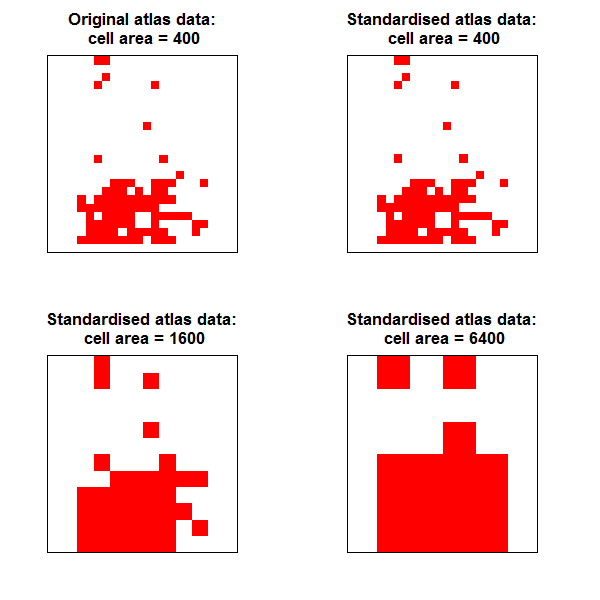
\includegraphics{Downscaling-downscale33}
\begin{Schunk}
\begin{Sinput}
> ## We can see there has not been much increase in extent
> occupancy$occupancy.orig[1, 2]
\end{Sinput}
\begin{Soutput}
[1] 147200

\end{Soutput}
\begin{Sinput}
> occupancy$extent.stand
\end{Sinput}
\begin{Soutput}
[1] 153600

\end{Soutput}
\end{Schunk}

Now we can run our ensemble downscaling models:

\setkeys{Gin}{width=1\linewidth}
\begin{Schunk}
\begin{Sinput}
> ensemble <- ensemble.downscale(occupancy,
+                                models = "all",
+                                new.areas = c(1, 10, 100, 400, 1600, 6400),
+                                tolerance_mod = 1e-3)
\end{Sinput}
\begin{Soutput}
Nachman model is running...  complete 
PL model is running...  complete 
Logis model is running...  complete 
Poisson model is running...  complete 
NB model is running...  complete 
GNB model is running...  complete 
INB model is running...  complete 
FNB model is running...  complete 
Thomas model is running...  complete 
Hui model is running...  complete 

\end{Soutput}
\end{Schunk}
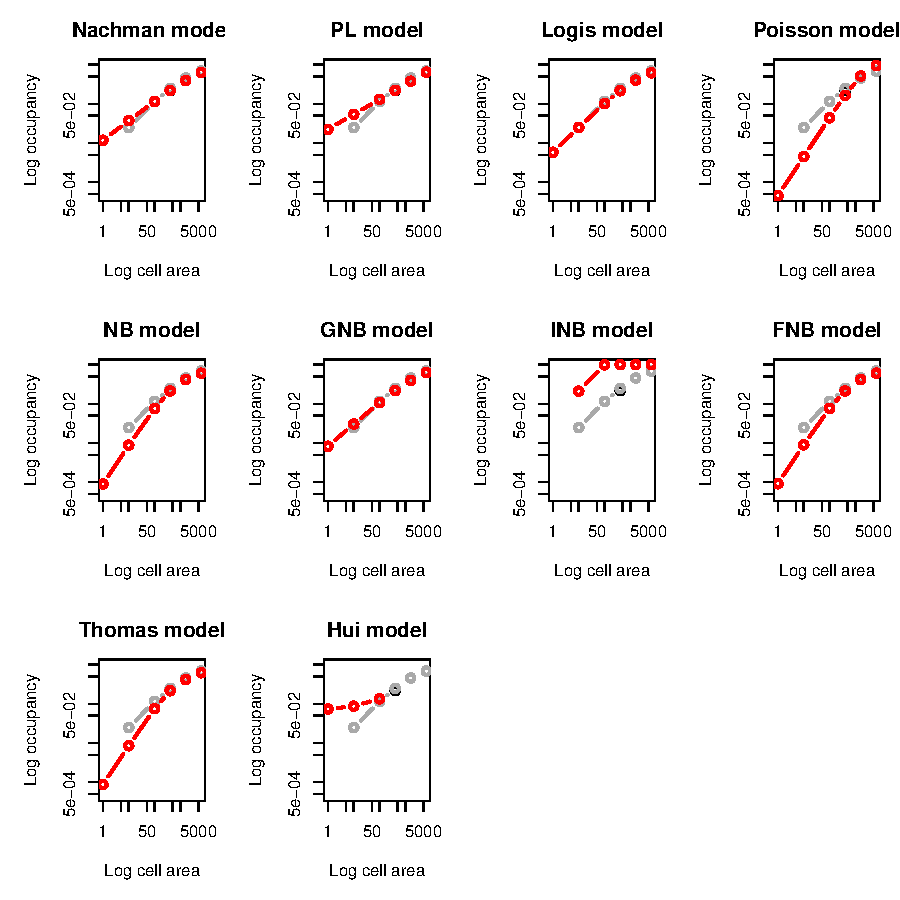
\includegraphics{Downscaling-downscale35}

The INB model has not converged satisfactorily and thrown up a warning message (it has predicted a 0 at the finest grain size which we know to be impossible). We can try tweaking it’s starting parameters to see if we can get a better fit:

\begin{Schunk}
\begin{Sinput}
> ensemble <- ensemble.downscale(occupancy,
+                                models = "all",
+                                new.areas = c(1, 10, 100, 400, 1600, 6400),
+                                tolerance_mod = 1e-3,
+                                starting_params = list(INB = list(C = 00.1, 
+                                                                  r = 0.01, 
+                                                                  b = 0.1)))
\end{Sinput}
\begin{Soutput}
Nachman model is running...  complete 
PL model is running...  complete 
Logis model is running...  complete 
Poisson model is running...  complete 
NB model is running...  complete 
GNB model is running...  complete 
INB model is running...  complete 
FNB model is running...  complete 
Thomas model is running...  complete 
Hui model is running...  complete 

\end{Soutput}
\end{Schunk}
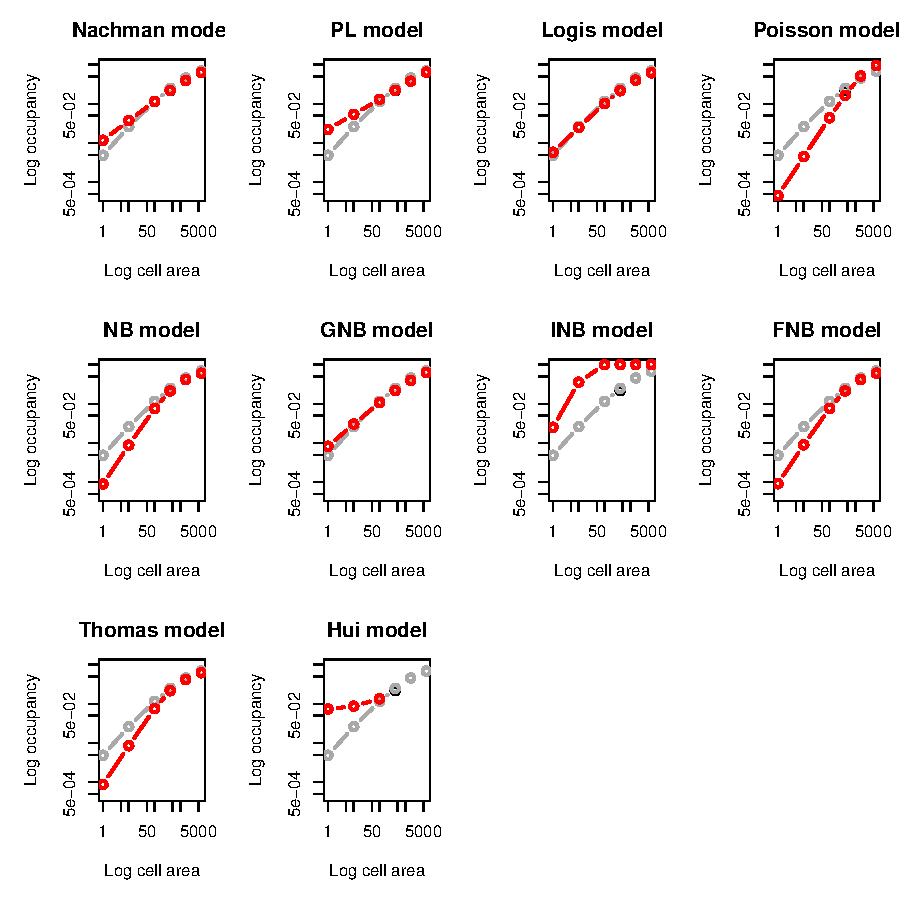
\includegraphics{Downscaling-downscale36}

In this case we have simply drawn a rectangle around our points, but perhaps we have a better idea of the possible range limits of the species. In our case, it is probably sensible to set the extent as mainland UK. There is a shapefile which we can load in and set as our extent.

\begin{Schunk}
\begin{Sinput}
> uk <- system.file("extdata", "UK.shp", package = "downscale")
> uk <- shapefile(uk)
> ## coverts units to be the same as our GBIF data (in km)
> uk <- spTransform(uk,
+                   CRS("+proj=lcc +lat_1=49.8333339 +lat_2=51.16666733333333 
+                       +lat_0=90 +lon_0=4.367486666666666 +x_0=150000.01256 
+                       +y_0=5400088.4378 +ellps=intl +units=km +no_defs"))
\end{Sinput}
\end{Schunk}

\setkeys{Gin}{width=0.8\linewidth}
\begin{Schunk}
\begin{Sinput}
> ## plot our GBIF records on top of the UK polygon
> plot(uk)
> plot(records, add = TRUE)
\end{Sinput}
\end{Schunk}
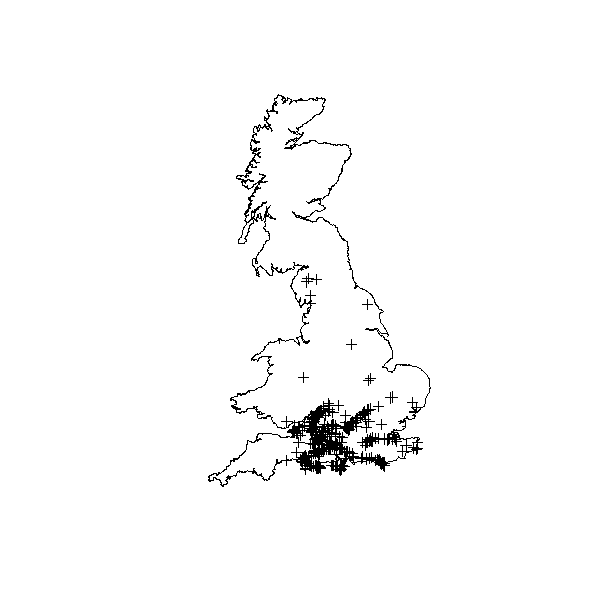
\includegraphics{Downscaling-downscale38}

Now, we make our raster to be the same extent as the UK polygon, and then mask the raster file with the UK polygon so that any cells outside this polygon are assigned as NA (unsampled cells):

\begin{Schunk}
\begin{Sinput}
> gbif_raster <- raster(ext = extent(uk),
+                       res = 20)
> gbif_raster <- rasterize(records, gbif_raster, field = 1)
> gbif_raster[is.na(gbif_raster)] <- 0
> gbif_raster <- mask(gbif_raster, uk)
\end{Sinput}
\end{Schunk}
\begin{Schunk}
\begin{Sinput}
> plot(gbif_raster)
> plot(uk, add = TRUE)
\end{Sinput}
\end{Schunk}
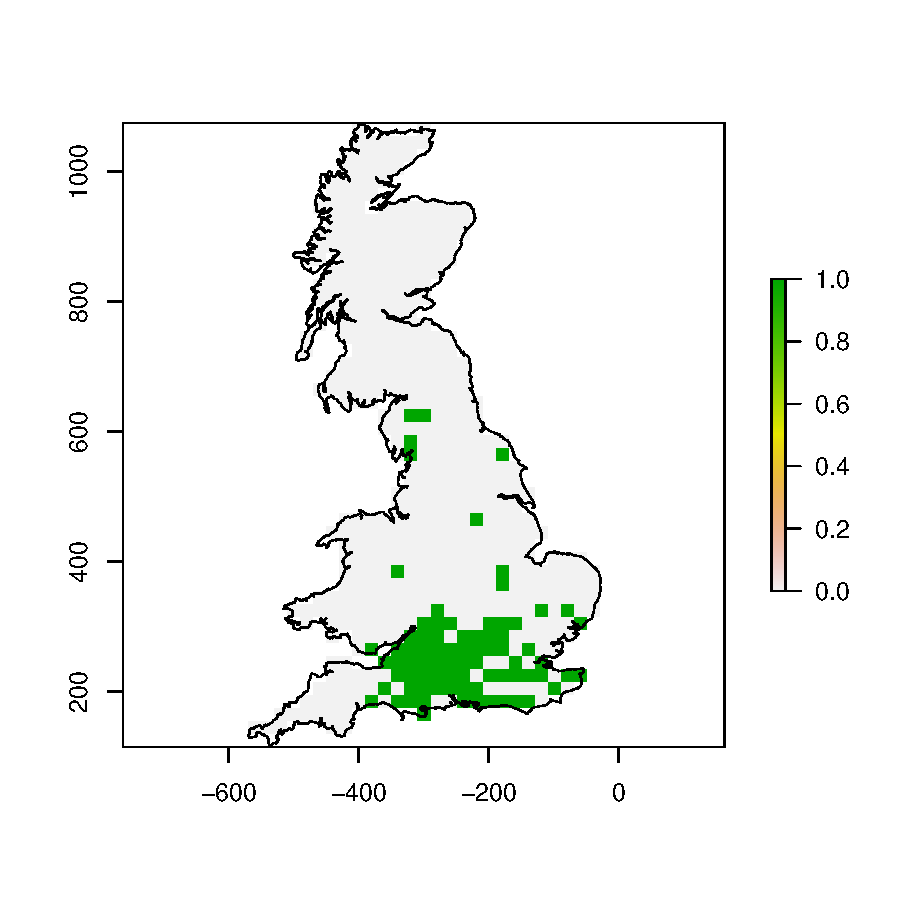
\includegraphics{Downscaling-downscale40}

Now, we just upgrain and downscale as before:

\begin{Schunk}
\begin{Sinput}
> occupancy <- upgrain(gbif_raster,
+                      scales = 2,
+                      method = "All_Sampled")
\end{Sinput}
\end{Schunk}
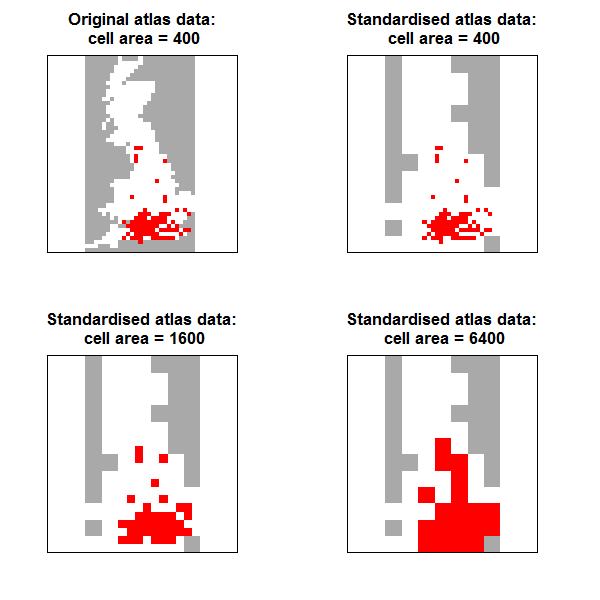
\includegraphics{Downscaling-downscale41}
\setkeys{Gin}{width=1\linewidth}
\begin{Schunk}
\begin{Sinput}
> ensemble.downscale(occupancy,
+                    models = "all",
+                    new.areas = c(1, 10, 100, 400, 1600, 6400),
+                    tolerance_mod = 1e-3,
+                    starting_params = list(INB = list(C = 10,
+                                                      r = 0.01,
+                                                      b = 0.1)))
\end{Sinput}
\begin{Soutput}
Nachman model is running...  complete 
PL model is running...  complete 
Logis model is running...  complete 
Poisson model is running...  complete 
NB model is running...  complete 
GNB model is running...  complete 
INB model is running...  complete 
FNB model is running...  complete 
Thomas model is running...  complete 
Hui model is running...  complete 
$Occupancy
  Cell.area     Nachman          PL      Logis      Poisson
1         1 0.003574872 0.004720191 0.00268301 0.0001365129
2        10 0.012295747 0.014454274 0.01042208 0.0013642906
3       100 0.041839989 0.044262197 0.03959798 0.0135594518
4       400 0.086210319 0.086827282 0.08573215 0.0531445930
5      1600 0.173180215 0.170325414 0.17577808 0.1962247036
6      6400 0.330438881 0.334120174 0.32661407 0.5826132897
            NB         GNB         INB          FNB
1 0.0003038185 0.003573846 0.003413519 0.0003084653
2 0.0030044948 0.012293650 0.012060053 0.0030488420
3 0.0271216798 0.041837325 0.041665287 0.0274028922
4 0.0835920937 0.086209204 0.086227000 0.0838010248
5 0.1882913465 0.173182594 0.173436297 0.1874537560
6 0.3128847147 0.330437696 0.330522529 0.3131943391
        Thomas        Hui       Means
1 0.0004386724 0.02611997 0.001551775
2 0.0042863249 0.03144745 0.007353972
3 0.0349979327 0.05133530 0.034391011
4 0.0889687100         NA 0.081463488
5 0.1740512870         NA 0.178902245
6 0.3400108394         NA 0.348818071

$AOO
  Cell.area    Nachman         PL       Logis      Poisson
1         1   1281.234   1691.716    961.5907     48.92622
2        10   4406.796   5180.412   3735.2743    488.96174
3       100  14995.452  15863.571  14191.9169   4859.70751
4       400  30897.778  31118.898  30726.4033  19047.02212
5      1600  62067.789  61044.628  62998.8645  70326.93378
6      6400 118429.295 119748.671 117058.4813 208808.60301
           NB        GNB        INB        FNB      Thomas
1    108.8886   1280.866   1223.405    110.554    157.2202
2   1076.8109   4406.044   4322.323   1092.705   1536.2188
3   9720.4100  14994.497  14932.839   9821.197  12543.2591
4  29959.4064  30897.379  30903.757  30034.287  31886.3857
5  67483.6186  62068.642  62159.569  67183.426  62379.9813
6 112137.8818 118428.870 118459.274 112248.851 121859.8849
        Hui       Means
1  9361.398    556.1562
2 11270.767   2635.6635
3 18398.570  12325.7384
4        NA  29196.5141
5        NA  64118.5645
6        NA 125016.3965


\end{Soutput}
\end{Schunk}
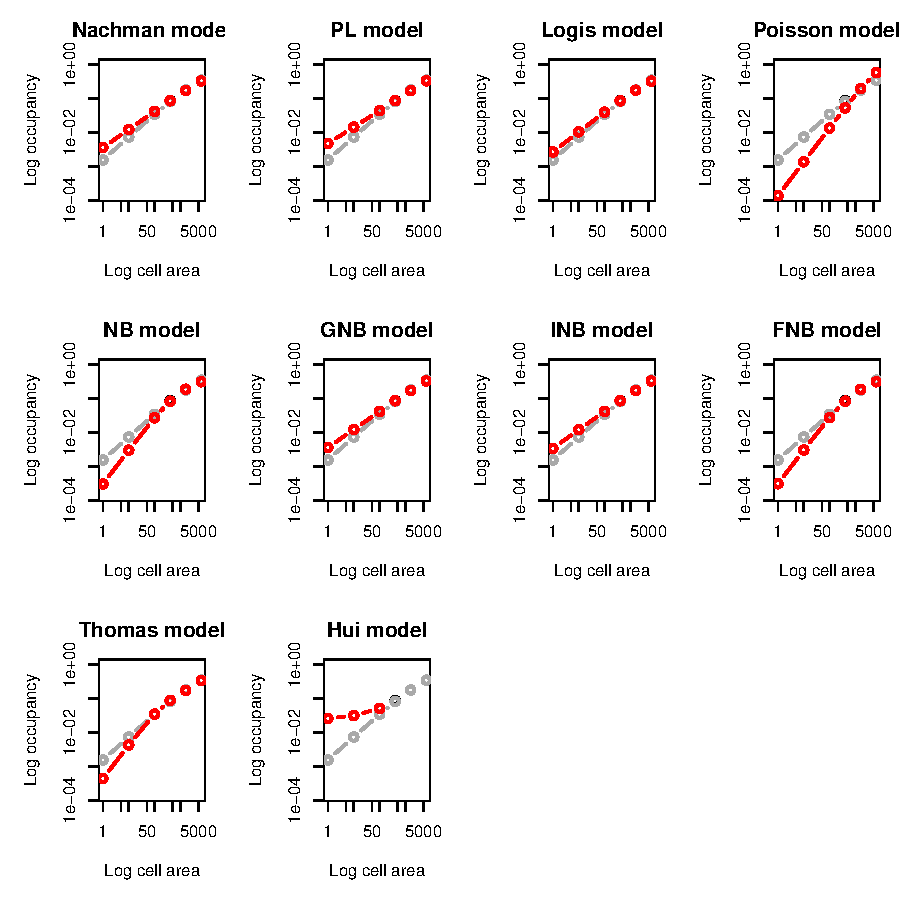
\includegraphics{Downscaling-downscale42}

If we want to compare occupancy between the two raster extents we must compare the converted area of occupancies (AOO), no proportion of occupancy (which are the proportions for different extents). In this case the estimates for grain sizes of 1 km and 10 km from the bounded rectangle (AOO = 627 $km^{2}$ and 3052 $km^{2}$) are larger than the estimates using the full mainland UK (AOO = 556 km^{2} and 2635 km^{2}) highlighting the importance of this decision.

\section{Bibliography}

Azaele, S., S. J. Cornell, and W. E. Kunin. 2012. Downscaling species occupancy from coarse spatial scales. Ecological Applications 22:1004–14.

Barwell, L. J., S. Azaele, W. E. Kunin, and N. J. B. Isaac. 2014. Can coarse-grain patterns in insect atlas data predict local occupancy? Diversity and Distributions 20:895–907.

Hartley, S., and W. E. Kunin. 2003. Scale dependence of rarity, extincition risk, and conservation priority. Conservation Biology 17:1–12.

Hui, C., M. A. McGeoch, B. Reyers, P. C. le Roux, M. Greve, and S. L. Chown. 2009. Extrapolating population size from the occupancy-abundance relationship and the scaling pattern of occupancy. Ecological Applications 19:2038–2048.

Hui, C., M. A. McGeoch, and M. Warren. 2006. A spatially explicit approach to estimating species occupancy and spatial correlation. Journal of Animal Ecology 75:140–147.

IUCN. 2014. Guidelines for using the IUCN Red List categories and criteria.

Kunin, W. E. 1998. Extrapolating species abundance across spatial scales. Science 281:1513–1515.

\end{document}
